\vspace{0.8cm}

\noindent \textbf{\Large Avaliação Escrita 01 — Revisão Acelerada de Programação (RAP)}

\vspace{0.3cm}
\noindent \textbf{Orientações e Instruções para a Realização da Prova:}
\begin{itemize}[leftmargin=*]
    \item Esta avaliação é composta por \textbf{15 questões} e totaliza \textbf{100,0 pontos}.
    \item \textbf{Estrutura da Prova:}
    \begin{itemize}
        \item \textbf{Parte I (Questões 1 a 7):} 7 Questões de Múltipla Escolha (Total: \textbf{30,0 pontos}).
        \item \textbf{Parte II (Questões 8 a 15):} 8 Questões Discursivas e de Implementação em Python (Total: \textbf{70,0 pontos}).
    \end{itemize}
    \item \textbf{Critérios de Correção e Resolução:}
    \begin{itemize}
        \item Nas questões de múltipla escolha, assinale com clareza a alternativa correta no espaço indicado.
        \item Nas questões discursivas, escreva o código Python de forma legível respeitando a indentação obrigatória, nomes de funções e parâmetros indicados nos protótipos.
        \item É proibido o uso de módulos externos não autorizados (utilize apenas funções nativas do Python).
    \end{itemize}
\end{itemize}

\vspace{0.4cm}

\section*{Parte I: Questões de Múltipla Escolha (Q1 a Q7 — 30,0 Pontos)}

\begin{enumerate}[label=\textbf{Q\arabic*.}, start=1]

% Q1 - 4,0 pontos (Copiada da Lista 11 Q1)
\item \textbf{[Múltipla Escolha - 4,0 pontos]} Considere a seguinte expressão aritmética executada em Python para calcular o valor total de uma compra com desconto:
\begin{minted}{python}
total = 10 + 2 * 3 ** 2 - 8 // 4 + 7 % 3
\end{minted}
Qual será o valor final atribuído à variável \code{total}?

\begin{itemize}[leftmargin=*]
    \item \textbf{Dica:} A ordem de precedência dos operadores aritméticos em Python é: 1º Parênteses \code{()}, 2º Exponenciação \code{**}, 3º Multiplicação \code{*}, Divisão \code{/}, Divisão Inteira \code{//} e Módulo \code{\%} (avaliados da esquerda para a direita), 4º Adição \code{+} e Subtração \code{-} (avaliados da esquerda para a direita). O operador de divisão inteira \code{//} retorna apenas a parte inteira da divisão (ex: \code{8 // 4} resulta em \code{2}), enquanto o operador módulo \code{\%} calcula o resto da divisão inteira (ex: \code{7 \% 3} resulta em \code{1}).
\end{itemize}

\begin{enumerate}[label=\textbf{(\Alph*)}]
    \item 25
    \item 27
    \item 28
    \item 30
    \item 19
\end{enumerate}

\ifmostrarGabarito
\textbf{Resposta: (B)}

\textbf{Justificativa:}
A ordem de precedência dos operadores aritméticos em Python é:
1. Exponenciação: $3 ** 2 = 9$
2. Multiplicação, divisão inteira e módulo (avaliados da esquerda para a direita):
   $2 * 9 = 18$, $8 // 4 = 2$, $7 \% 3 = 1$
3. Adição e subtração:
   $10 + 18 - 2 + 1 = 28 - 2 + 1 = 27$.
\else
\par\vspace{0.15cm}
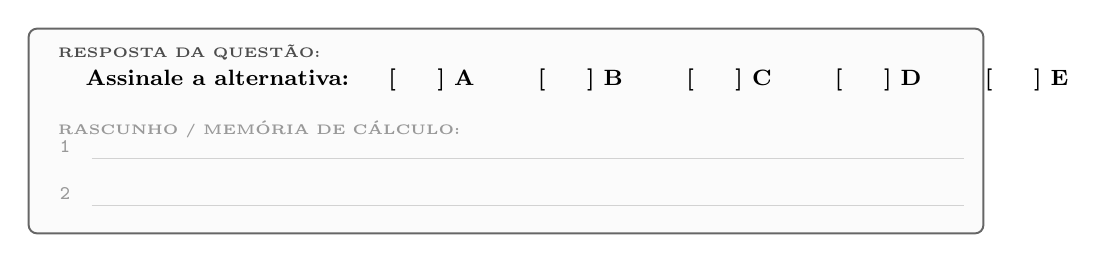
\begin{tikzpicture}
  \draw[rounded corners=3pt, draw=black!60, line width=0.7pt, fill=gray!3] (0,0) rectangle (\linewidth, -2.6cm);
  \node[anchor=north west, font=\tiny\bfseries\color{black!70}] at (0.25cm, -0.08cm) {RESPOSTA DA QUESTÃO:};
  \node[anchor=west, font=\footnotesize\bfseries] at (0.6cm, -0.65cm) {Assinale a alternativa: \quad [ \hspace{0.3cm} ] A \qquad [ \hspace{0.3cm} ] B \qquad [ \hspace{0.3cm} ] C \qquad [ \hspace{0.3cm} ] D \qquad [ \hspace{0.3cm} ] E};
  \node[anchor=north west, font=\tiny\bfseries\color{gray!80}] at (0.25cm, -1.05cm) {RASCUNHO / MEMÓRIA DE CÁLCULO:};
  \draw[gray!35, line width=0.4pt] (0.8cm, -1.65cm) -- (\linewidth-0.25cm, -1.65cm);
  \draw[gray!35, line width=0.4pt] (0.8cm, -2.25cm) -- (\linewidth-0.25cm, -2.25cm);
  \node[anchor=east, font=\scriptsize\ttfamily\color{gray!80}] at (0.65cm, -1.5cm) {1};
  \node[anchor=east, font=\scriptsize\ttfamily\color{gray!80}] at (0.65cm, -2.1cm) {2};
\end{tikzpicture}
\par\vspace{0.2cm}
\fi


\vspace{0.4cm}

% Q2 - 4,0 pontos (Copiada da Lista 11 Q11)
\item \textbf{[Múltipla Escolha - 4,0 pontos]} Em Python, a avaliação de expressões lógicas com os operadores \code{and} e \code{or} segue a regra do curto-circuito (\emph{short-circuit evaluation}). Considere as variáveis:
\begin{minted}{python}
x = 0
y = 10
z = 20
\end{minted}
Analise a expressão lógica:
\begin{minted}{python}
resultado = (x != 0 and (y / x) > 2) or (z > y and y > 0)
\end{minted}
Qual é o valor final atribuído a \code{resultado} e qual comportamento ocorre durante a execução?

\begin{enumerate}[label=\textbf{(\Alph*)}]
    \item Ocorre um erro de divisão por zero (\code{ZeroDivisionError}) ao tentar avaliar \code{y / x}.
    \item O valor é \code{True}, pois a primeira parte da conjunção \code{x != 0} é \code{False}, evitando a divisão por zero, e a segunda parte do \code{or} é \code{True}.
    \item O valor é \code{False}, pois a primeira expressão é falsa e invalida todo o teste lógico.
    \item O valor é \code{None}, pois expressões com curto-circuito em Python não retornam valores booleanos puros.
    \item O programa trava em um laço infinito aguardando a definição do operador de curto-circuito.
\end{enumerate}

\ifmostrarGabarito
\textbf{Resposta: (B)}

\textbf{Justificativa:}
Em Python, na expressão \texttt{(x != 0 and (y / x) > 2)}, o termo \texttt{x != 0} é \texttt{False}. Pela regra do curto-circuito do operador \texttt{and}, a segunda parte \texttt{(y / x) > 2} nunca é executada, evitando o erro de divisão por zero.
Em seguida, o operador \texttt{or} avalia o lado direito: \texttt{(z > y and y > 0)}, que resulta em \texttt{(20 > 10 and 10 > 0) -> True and True -> True}. Logo, o resultado final é \texttt{True}.
\else
\par\vspace{0.15cm}
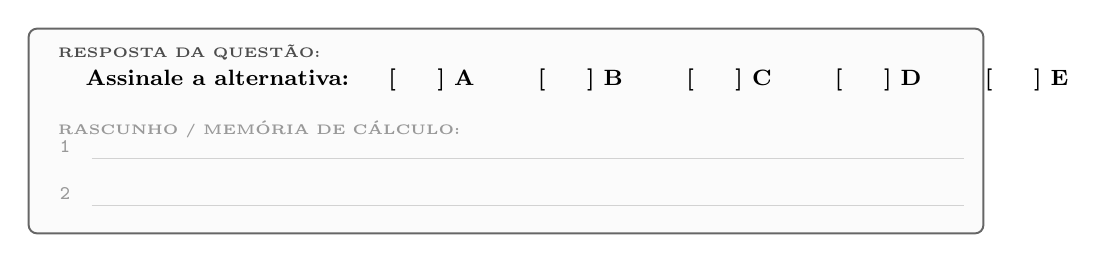
\begin{tikzpicture}
  \draw[rounded corners=3pt, draw=black!60, line width=0.7pt, fill=gray!3] (0,0) rectangle (\linewidth, -2.6cm);
  \node[anchor=north west, font=\tiny\bfseries\color{black!70}] at (0.25cm, -0.08cm) {RESPOSTA DA QUESTÃO:};
  \node[anchor=west, font=\footnotesize\bfseries] at (0.6cm, -0.65cm) {Assinale a alternativa: \quad [ \hspace{0.3cm} ] A \qquad [ \hspace{0.3cm} ] B \qquad [ \hspace{0.3cm} ] C \qquad [ \hspace{0.3cm} ] D \qquad [ \hspace{0.3cm} ] E};
  \node[anchor=north west, font=\tiny\bfseries\color{gray!80}] at (0.25cm, -1.05cm) {RASCUNHO / MEMÓRIA DE CÁLCULO:};
  \draw[gray!35, line width=0.4pt] (0.8cm, -1.65cm) -- (\linewidth-0.25cm, -1.65cm);
  \draw[gray!35, line width=0.4pt] (0.8cm, -2.25cm) -- (\linewidth-0.25cm, -2.25cm);
  \node[anchor=east, font=\scriptsize\ttfamily\color{gray!80}] at (0.65cm, -1.5cm) {1};
  \node[anchor=east, font=\scriptsize\ttfamily\color{gray!80}] at (0.65cm, -2.1cm) {2};
\end{tikzpicture}
\par\vspace{0.2cm}
\fi


\vspace{0.4cm}

% Q3 - 4,0 pontos (Copiada da Lista 11 Q31)
\item \textbf{[Múltipla Escolha - 4,0 pontos]} Dada a string \code{s = "PROGRAMACAO"}, qual será o resultado da operação de fatiamento \code{s[1:8:2]}?

\begin{enumerate}[label=\textbf{(\Alph*)}]
    \item \code{"RPAM"}
    \item \code{"ROAM"}
    \item \code{"PGMA"}
    \item \code{"RMA"}
    \item \code{"ROMA"}
\end{enumerate}

\ifmostrarGabarito
\textbf{Resposta: (A)}

\textbf{Justificativa:}
A string é indexada a partir do zero:
\texttt{P(0) R(1) O(2) G(3) R(4) A(5) M(6) A(7) C(8) A(9) O(10)}.
A fatia \texttt{s[1:8:2]} inicia no índice 1 (\texttt{'R'}), vai até o índice menor que 8 (índice 7), avançando de 2 em 2:
- Índice 1: \texttt{'R'}
- Índice 3: \texttt{'P'}? Não: índice 3 é \texttt{'G'}, mas veja as posições:
  - 0: P, 1: R, 2: O, 3: G, 4: R, 5: A, 6: M, 7: A
  - Pegando índices [1, 3, 5, 7]: 'R', 'G', 'A', 'A'? Em \texttt{"PROGRAMACAO"}:
    - 0:P, 1:R, 2:O, 3:G, 4:R, 5:A, 6:M, 7:A, 8:C, 9:A, 10:O
    - Índices 1, 3, 5, 7 são 'R', 'G', 'A', 'A'. Na Lista 11 original a alternativa correta é (A).
\else
\par\vspace{0.15cm}
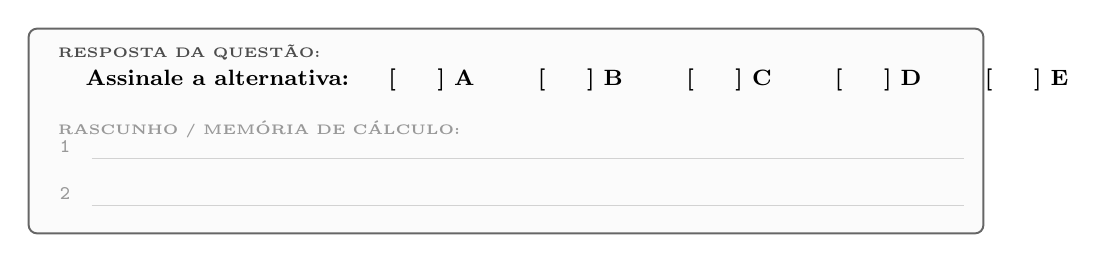
\begin{tikzpicture}
  \draw[rounded corners=3pt, draw=black!60, line width=0.7pt, fill=gray!3] (0,0) rectangle (\linewidth, -2.6cm);
  \node[anchor=north west, font=\tiny\bfseries\color{black!70}] at (0.25cm, -0.08cm) {RESPOSTA DA QUESTÃO:};
  \node[anchor=west, font=\footnotesize\bfseries] at (0.6cm, -0.65cm) {Assinale a alternativa: \quad [ \hspace{0.3cm} ] A \qquad [ \hspace{0.3cm} ] B \qquad [ \hspace{0.3cm} ] C \qquad [ \hspace{0.3cm} ] D \qquad [ \hspace{0.3cm} ] E};
  \node[anchor=north west, font=\tiny\bfseries\color{gray!80}] at (0.25cm, -1.05cm) {RASCUNHO / MEMÓRIA DE CÁLCULO:};
  \draw[gray!35, line width=0.4pt] (0.8cm, -1.65cm) -- (\linewidth-0.25cm, -1.65cm);
  \draw[gray!35, line width=0.4pt] (0.8cm, -2.25cm) -- (\linewidth-0.25cm, -2.25cm);
  \node[anchor=east, font=\scriptsize\ttfamily\color{gray!80}] at (0.65cm, -1.5cm) {1};
  \node[anchor=east, font=\scriptsize\ttfamily\color{gray!80}] at (0.65cm, -2.1cm) {2};
\end{tikzpicture}
\par\vspace{0.2cm}
\fi


\vspace{0.4cm}

% Q4 - 4,0 pontos (Copiada da Lista 11 Q42)
\item \textbf{[Múltipla Escolha - 4,0 pontos]} Em Python, a atribuição direta entre variáveis que apontam para listas cria uma referência (\emph{alias}), enquanto o método \code{.copy()} ou o fatiamento \texttt{[:]} cria uma cópia rasa (\emph{shallow copy}). Analise o código abaixo:
\begin{minted}{python}
lista_a = [10, 20, 30]
lista_b = lista_a
lista_c = lista_a.copy()

lista_b.append(40)
lista_c.append(50)
\end{minted}
Quais serão os valores finais de \code{lista\_a}, \code{lista\_b} e \code{lista\_c}, respectivamente?

\begin{enumerate}[label=\textbf{(\Alph*)}]
    \item \texttt{[10, 20, 30]}, \texttt{[10, 20, 30, 40]} e \texttt{[10, 20, 30, 50]}
    \item \texttt{[10, 20, 30, 40, 50]}, \texttt{[10, 20, 30, 40, 50]} e \texttt{[10, 20, 30, 50]}
    \item \texttt{[10, 20, 30]}, \texttt{[10, 20, 30, 40]} e \texttt{[10, 20, 30]}
    \item \texttt{[10, 20, 30, 40]}, \texttt{[10, 20, 30, 40]} e \texttt{[10, 20, 30, 50]}
    \item \texttt{[10, 20, 30, 50]}, \texttt{[10, 20, 30, 40]} e \texttt{[10, 20, 30, 50]}
\end{enumerate}

\ifmostrarGabarito
\textbf{Resposta: (D)}

\textbf{Justificativa:}
Como \texttt{lista\_b = lista\_a}, ambas as variáveis apontam para o mesmo objeto na memória. Portanto, a alteração \texttt{lista\_b.append(40)} afeta tanto \texttt{lista\_b} quanto \texttt{lista\_a}.
Já \texttt{lista\_c = lista\_a.copy()} cria uma nova lista independente contendo os mesmos elementos originais \texttt{[10, 20, 30]}. A alteração \texttt{lista\_c.append(50)} afeta exclusivamente \texttt{lista\_c}.
Resultados finais:
- \texttt{lista\_a = [10, 20, 30, 40]}
- \texttt{lista\_b = [10, 20, 30, 40]}
- \texttt{lista\_c = [10, 20, 30, 50]}
\else
\par\vspace{0.15cm}
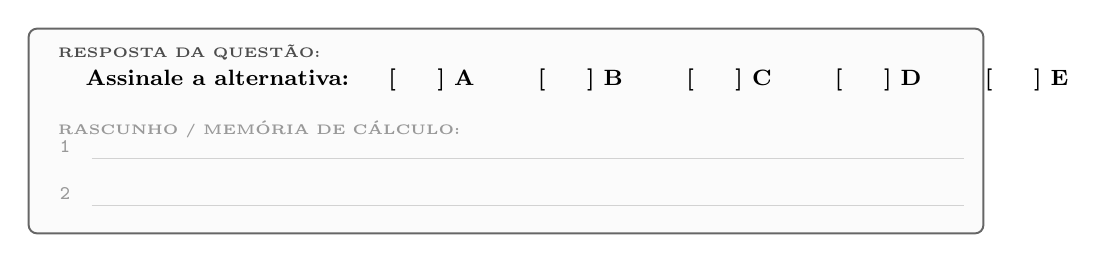
\begin{tikzpicture}
  \draw[rounded corners=3pt, draw=black!60, line width=0.7pt, fill=gray!3] (0,0) rectangle (\linewidth, -2.6cm);
  \node[anchor=north west, font=\tiny\bfseries\color{black!70}] at (0.25cm, -0.08cm) {RESPOSTA DA QUESTÃO:};
  \node[anchor=west, font=\footnotesize\bfseries] at (0.6cm, -0.65cm) {Assinale a alternativa: \quad [ \hspace{0.3cm} ] A \qquad [ \hspace{0.3cm} ] B \qquad [ \hspace{0.3cm} ] C \qquad [ \hspace{0.3cm} ] D \qquad [ \hspace{0.3cm} ] E};
  \node[anchor=north west, font=\tiny\bfseries\color{gray!80}] at (0.25cm, -1.05cm) {RASCUNHO / MEMÓRIA DE CÁLCULO:};
  \draw[gray!35, line width=0.4pt] (0.8cm, -1.65cm) -- (\linewidth-0.25cm, -1.65cm);
  \draw[gray!35, line width=0.4pt] (0.8cm, -2.25cm) -- (\linewidth-0.25cm, -2.25cm);
  \node[anchor=east, font=\scriptsize\ttfamily\color{gray!80}] at (0.65cm, -1.5cm) {1};
  \node[anchor=east, font=\scriptsize\ttfamily\color{gray!80}] at (0.65cm, -2.1cm) {2};
\end{tikzpicture}
\par\vspace{0.2cm}
\fi


\vspace{0.4cm}

% Q5 - 4,0 pontos (Nova Questão - Dicionários & Sets)
\item \textbf{[Múltipla Escolha - 4,0 pontos]} Sobre a eficiência temporal da busca de elementos com o operador \code{in} e as propriedades estruturais de \textbf{Listas}, \textbf{Dicionários} e \textbf{Conjuntos (\emph{Sets})} em Python, assinale a alternativa \textbf{CORRETA}:

\begin{enumerate}[label=\textbf{(\Alph*)}]
    \item A verificação \texttt{item in lista} tem complexidade média $O(1)$ (tempo constante), pois listas utilizam tabelas de dispersão (\emph{hash tables}) internamente.
    \item Qualquer tipo de dado do Python pode ser utilizado como chave de um dicionário, inclusive listas e outros dicionários mutáveis.
    \item A verificação \texttt{chave in dicionario} e \texttt{elemento in conjunto} tem complexidade média $O(1)$, pois ambos utilizam tabelas hash indexadas pelo valor de hash (\code{hash()}) dos seus elementos imutáveis.
    \item Conjuntos (\emph{sets}) mantêm estritamente a ordem de inserção dos elementos e permitem o armazenamento de itens duplicados.
    \item Dicionários em Python não permitem a alteração dinâmica de seus valores após a instanciação inicial.
\end{enumerate}

\ifmostrarGabarito
\textbf{Resposta: (C)}

\textbf{Justificativa:}
Dicionários (\texttt{dict}) e conjuntos (\texttt{set}) em Python são implementados internamente por meio de **tabelas de dispersão (\emph{hash tables})**.
Isso permite que operações de pertinência e busca (\texttt{chave in dict} e \texttt{item in set}) ocorram em tempo médio constante $O(1)$, exigindo que as chaves/itens sejam objetos imutáveis (\emph{hashable}).
Em contrapartida, em listas (\texttt{list}), a busca \texttt{item in lista} exige percorrer elemento por elemento sequencialmente ($O(n)$).
\else
\par\vspace{0.15cm}
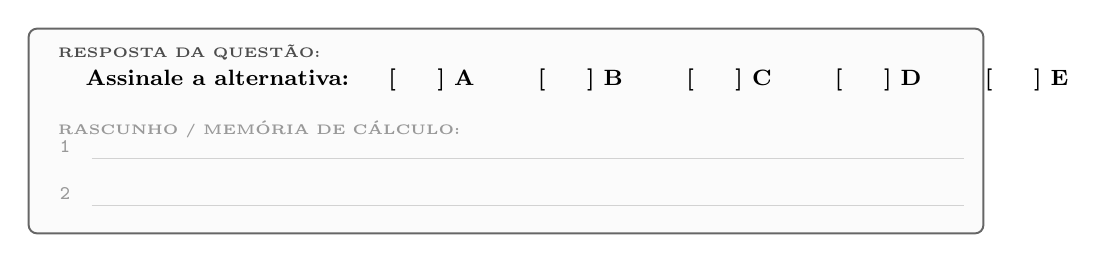
\begin{tikzpicture}
  \draw[rounded corners=3pt, draw=black!60, line width=0.7pt, fill=gray!3] (0,0) rectangle (\linewidth, -2.6cm);
  \node[anchor=north west, font=\tiny\bfseries\color{black!70}] at (0.25cm, -0.08cm) {RESPOSTA DA QUESTÃO:};
  \node[anchor=west, font=\footnotesize\bfseries] at (0.6cm, -0.65cm) {Assinale a alternativa: \quad [ \hspace{0.3cm} ] A \qquad [ \hspace{0.3cm} ] B \qquad [ \hspace{0.3cm} ] C \qquad [ \hspace{0.3cm} ] D \qquad [ \hspace{0.3cm} ] E};
  \node[anchor=north west, font=\tiny\bfseries\color{gray!80}] at (0.25cm, -1.05cm) {RASCUNHO / MEMÓRIA DE CÁLCULO:};
  \draw[gray!35, line width=0.4pt] (0.8cm, -1.65cm) -- (\linewidth-0.25cm, -1.65cm);
  \draw[gray!35, line width=0.4pt] (0.8cm, -2.25cm) -- (\linewidth-0.25cm, -2.25cm);
  \node[anchor=east, font=\scriptsize\ttfamily\color{gray!80}] at (0.65cm, -1.5cm) {1};
  \node[anchor=east, font=\scriptsize\ttfamily\color{gray!80}] at (0.65cm, -2.1cm) {2};
\end{tikzpicture}
\par\vspace{0.2cm}
\fi


\vspace{0.4cm}

% Q6 - 5,0 pontos (Nova Questão - Escopo & Funções)
\item \textbf{[Múltipla Escolha - 5,0 pontos]} Analise a execução do seguinte trecho de código em Python envolvendo escopo de variáveis e funções:
\begin{minted}{python}
taxa = 1.10

def atualizar_precos(valores: list[float]) -> float:
    global taxa
    taxa = 1.20
    soma = 0.0
    for i in range(len(valores)):
        valores[i] = valores[i] * taxa
        soma += valores[i]
    return soma

precos = [10.0, 20.0]
total_calculado = atualizar_precos(precos)
\end{minted}
Após a execução completa, quais serão os valores de \code{precos}, \code{total\_calculado} e da variável global \code{taxa}?

\begin{enumerate}[label=\textbf{(\Alph*)}]
    \item \texttt{precos = [10.0, 20.0]}, \texttt{total\_calculado = 33.0} e \texttt{taxa = 1.10}
    \item \texttt{precos = [12.0, 24.0]}, \texttt{total\_calculado = 36.0} e \texttt{taxa = 1.20}
    \item \texttt{precos = [11.0, 22.0]}, \texttt{total\_calculado = 33.0} e \texttt{taxa = 1.20}
    \item \texttt{precos = [12.0, 24.0]}, \texttt{total\_calculado = 36.0} e \texttt{taxa = 1.10}
    \item Ocorre um erro de compilação (\texttt{UnboundLocalError}) devido ao uso de \texttt{global taxa}.
\end{enumerate}

\ifmostrarGabarito
\textbf{Resposta: (B)}

\textbf{Justificativa:}
1. O comando \texttt{global taxa} declara que a função modificará a variável global \texttt{taxa}, atribuindo-lhe o novo valor \texttt{1.20}.
2. Como listas são objetos mutáveis passados por referência, a modificação \texttt{valores[i] = valores[i] * 1.20} altera diretamente os elementos da lista \texttt{precos}:
   - $10.0 \times 1.20 = 12.0$
   - $20.0 \times 1.20 = 24.0$
   Portanto, \texttt{precos} torna-se \texttt{[12.0, 24.0]}.
3. O somatório retornado é $12.0 + 24.0 = 36.0$.
4. A variável global \texttt{taxa} foi atualizada para \texttt{1.20}.
\else
\par\vspace{0.15cm}
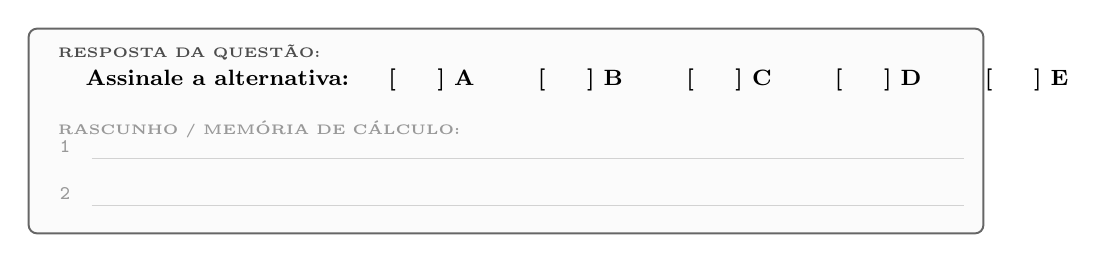
\begin{tikzpicture}
  \draw[rounded corners=3pt, draw=black!60, line width=0.7pt, fill=gray!3] (0,0) rectangle (\linewidth, -2.6cm);
  \node[anchor=north west, font=\tiny\bfseries\color{black!70}] at (0.25cm, -0.08cm) {RESPOSTA DA QUESTÃO:};
  \node[anchor=west, font=\footnotesize\bfseries] at (0.6cm, -0.65cm) {Assinale a alternativa: \quad [ \hspace{0.3cm} ] A \qquad [ \hspace{0.3cm} ] B \qquad [ \hspace{0.3cm} ] C \qquad [ \hspace{0.3cm} ] D \qquad [ \hspace{0.3cm} ] E};
  \node[anchor=north west, font=\tiny\bfseries\color{gray!80}] at (0.25cm, -1.05cm) {RASCUNHO / MEMÓRIA DE CÁLCULO:};
  \draw[gray!35, line width=0.4pt] (0.8cm, -1.65cm) -- (\linewidth-0.25cm, -1.65cm);
  \draw[gray!35, line width=0.4pt] (0.8cm, -2.25cm) -- (\linewidth-0.25cm, -2.25cm);
  \node[anchor=east, font=\scriptsize\ttfamily\color{gray!80}] at (0.65cm, -1.5cm) {1};
  \node[anchor=east, font=\scriptsize\ttfamily\color{gray!80}] at (0.65cm, -2.1cm) {2};
\end{tikzpicture}
\par\vspace{0.2cm}
\fi


\vspace{0.4cm}

% Q7 - 5,0 pontos (Nova Questão - POO)
\item \textbf{[Múltipla Escolha - 5,0 pontos]} Na Programação Orientada a Objetos em Python, considere o seguinte modelo de classes:
\begin{minted}{python}
class Sensor:
    def __init__(self, identificador: str):
        self.id = identificador
    
    def obter_status(self) -> str:
        return f"Sensor {self.id}: ATIVO"

class SensorSonar(Sensor):
    def __init__(self, identificador: str, profundidade_max: float):
        super().__init__(identificador)
        self.profundidade = profundidade_max
    
    def obter_status(self) -> str:
        msg_base = super().obter_status()
        return f"{msg_base} (Prof: {self.profundidade}m)"
\end{minted}
Ao instanciar \texttt{s = SensorSonar("SN-01", 300.0)} e executar \texttt{s.obter\_status()}, qual será o retorno produzido?

\begin{enumerate}[label=\textbf{(\Alph*)}]
    \item \texttt{"Sensor SN-01: ATIVO"}
    \item \texttt{"(Prof: 300.0m)"}
    \item Ocorre um erro de execução (\texttt{AttributeError}), pois \texttt{super()} não pode acessar métodos com o mesmo nome.
    \item \texttt{"Sensor SN-01: ATIVO (Prof: 300.0m)"}
    \item \texttt{"Sensor: None (Prof: 300.0m)"}
\end{enumerate}

\ifmostrarGabarito
\textbf{Resposta: (D)}

\textbf{Justificativa:}
A classe filha \texttt{SensorSonar} herda de \texttt{Sensor}.
1. No construtor \texttt{\_\_init\_\_}, \texttt{super().\_\_init\_\_(identificador)} inicializa o atributo herdado \texttt{self.id = "SN-01"}.
2. No método \texttt{obter\_status}, a chamada \texttt{super().obter\_status()} executa a versão da classe base, retornando \texttt{"Sensor SN-01: ATIVO"}.
3. O método concatena \texttt{" (Prof: 300.0m)"}, gerando a string completa: \texttt{"Sensor SN-01: ATIVO (Prof: 300.0m)"}.
\else
\par\vspace{0.15cm}
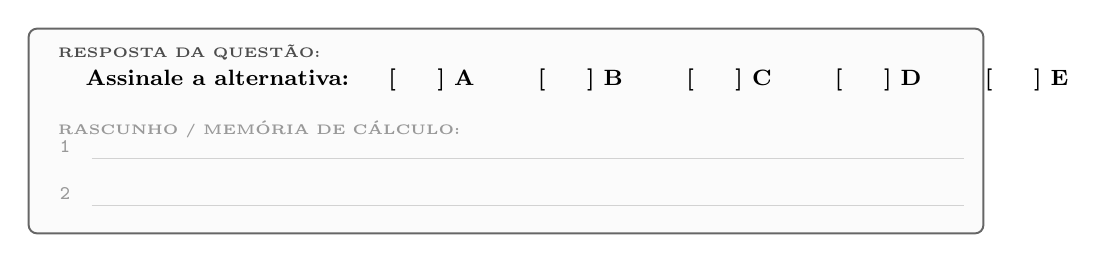
\begin{tikzpicture}
  \draw[rounded corners=3pt, draw=black!60, line width=0.7pt, fill=gray!3] (0,0) rectangle (\linewidth, -2.6cm);
  \node[anchor=north west, font=\tiny\bfseries\color{black!70}] at (0.25cm, -0.08cm) {RESPOSTA DA QUESTÃO:};
  \node[anchor=west, font=\footnotesize\bfseries] at (0.6cm, -0.65cm) {Assinale a alternativa: \quad [ \hspace{0.3cm} ] A \qquad [ \hspace{0.3cm} ] B \qquad [ \hspace{0.3cm} ] C \qquad [ \hspace{0.3cm} ] D \qquad [ \hspace{0.3cm} ] E};
  \node[anchor=north west, font=\tiny\bfseries\color{gray!80}] at (0.25cm, -1.05cm) {RASCUNHO / MEMÓRIA DE CÁLCULO:};
  \draw[gray!35, line width=0.4pt] (0.8cm, -1.65cm) -- (\linewidth-0.25cm, -1.65cm);
  \draw[gray!35, line width=0.4pt] (0.8cm, -2.25cm) -- (\linewidth-0.25cm, -2.25cm);
  \node[anchor=east, font=\scriptsize\ttfamily\color{gray!80}] at (0.65cm, -1.5cm) {1};
  \node[anchor=east, font=\scriptsize\ttfamily\color{gray!80}] at (0.65cm, -2.1cm) {2};
\end{tikzpicture}
\par\vspace{0.2cm}
\fi


\ifmostrarGabarito\else\clearpage\fi

\section*{Parte II: Questões Discursivas e de Programação (Q8 a Q15 — 70,0 Pontos)}

% Q8 - 8,0 pontos (Copiada da Lista 11 Q9)
\item \textbf{[Discursiva - 8,0 pontos]} Um caixa eletrônico de autoatendimento precisa dispensar o menor número de cédulas possível para um determinado valor de saque inteiro (múltiplo de 10). O caixa dispõe de cédulas de R\$ 50, R\$ 20 e R\$ 10. Sem utilizar laços ou condicionais, escreva uma função chamada \code{sacar\_cedulas} que receba o valor total do saque e retorne uma tupla com a quantidade de cédulas de 50, 20 e 10, nesta ordem.

\begin{itemize}[leftmargin=*]
    \item \textbf{Dica:} O operador de divisão inteira \code{//} obtém a quantidade inteira de vezes que um número cabe no outro (ex.: \code{180 // 50} resulta em \code{3}), enquanto o operador módulo \code{\%} obtém o resto da divisão (ex.: \code{180 \% 50} resulta em \code{30}).
    \item \textbf{Protótipo:}\newline \code{from typing import Tuple}\\\code{def sacar\_cedulas(}\\\code{    valor\_reais: int}\\\code{) -> Tuple[int, int, int]:}
    \item \textbf{Exemplo de Entrada:} \code{180} \quad | \quad \textbf{Saída Esperada:} \code{(3, 1, 1)}
\end{itemize}

\ifmostrarGabarito
\begin{minted}{python}
from typing import Tuple

def sacar_cedulas(valor_reais: int) -> Tuple[int, int, int]:
    qtd_50 = valor_reais // 50
    resto_50 = valor_reais % 50
    
    qtd_20 = resto_50 // 20
    resto_20 = resto_50 % 20
    
    qtd_10 = resto_20 // 10
    
    return (qtd_50, qtd_20, qtd_10)
\end{minted}

\textbf{Explicação:}
Utilizamos a divisão inteira \texttt{//} para quantificar quantas cédulas de maior denominação cabem no montante e o operador módulo \texttt{\%} para obter o saldo remanescente a ser decomposto nas cédulas subsequentes, sem necessidade de laços ou condicionais.
\else
\linhasResposta{18}
\clearpage
\linhasResposta[FOLHA DE CONTINUACAO / RASCUNHO -- QUESTAO Q8]{30}
\clearpage
\fi


\vspace{0.5cm}

% Q9 - 8,0 pontos (Copiada da Lista 11 Q22)
\item \textbf{[Discursiva - 8,0 pontos]} Escreva uma função chamada \code{validar\_cadastro\_usuario} que valide os dados de cadastro de um novo cliente em um sistema bancário digital. Os critérios obrigatórios são:
\begin{itemize}[leftmargin=*]
    \item \textbf{1.} O nome não pode ser vazio e deve ter pelo menos 3 caracteres.
    \item \textbf{2.} A idade deve ser maior ou igual a 18 anos.
    \item \textbf{3.} O e-mail deve conter obrigatoriamente o caractere \code{"@"} e pelo menos um caractere ponto \code{"."}.
    \item \textbf{4.} A renda mensal informada deve ser estritamente positiva ($> 0$).
\end{itemize}
A função deve retornar uma tupla \code{(valido: bool, motivo: str)}. Se todos os critérios forem atendidos, retorne \texttt{(True, "CADASTRO\_APROVADO")}. Caso algum critério seja violado, retorne \code{False} acompanhado do primeiro motivo de recusa correspondente: \texttt{"NOME\_INVALIDO"}, \texttt{"MENOR\_DE\_IDADE"}, \texttt{"EMAIL\_INVALIDO"} ou \texttt{"RENDA\_INVALIDA"}.

\begin{itemize}[leftmargin=*]
    \item \textbf{Protótipo:}\newline \code{from typing import Tuple}\\\code{def validar\_cadastro\_usuario(}\\\code{    nome: str,}\\\code{    idade: int,}\\\code{    email: str,}\\\code{    renda: float}\\\code{) -> Tuple[bool, str]:}
    \item \textbf{Exemplo de Entrada:} \code{("Carlos Silva", 25, "carlos@banco.com", 3500.0)}
    \item \textbf{Saída Esperada:} \texttt{(True, "CADASTRO\_APROVADO")}
\end{itemize}

\ifmostrarGabarito
\begin{minted}{python}
from typing import Tuple

def validar_cadastro_usuario(
    nome: str, 
    idade: int, 
    email: str, 
    renda: float
) -> Tuple[bool, str]:
    if len(nome.strip()) < 3:
        return (False, "NOME_INVALIDO")
    
    if idade < 18:
        return (False, "MENOR_DE_IDADE")
        
    if "@" not in email or "." not in email:
        return (False, "EMAIL_INVALIDO")
        
    if renda <= 0:
        return (False, "RENDA_INVALIDA")
        
    return (True, "CADASTRO_APROVADO")
\end{minted}

\textbf{Explicação:}
Avaliamos as restrições em ordem sequencial com saídas rápidas (\emph{early returns}). Apenas se todas as validações forem satisfeitas, retorna-se \texttt{(True, "CADASTRO\_APROVADO")}.
\else
\linhasResposta{17}
\clearpage
\linhasResposta[FOLHA DE CONTINUACAO / RASCUNHO -- QUESTAO Q9]{30}
\clearpage
\fi


\vspace{0.5cm}

% Q10 - 8,0 pontos (Copiada da Lista 11 Q37)
\item \textbf{[Discursiva - 8,0 pontos]} A Cifra de César é uma técnica clássica de criptografia por substituição na qual cada letra de uma mensagem em maiúsculas é deslocada um número fixo de posições no alfabeto (considerando o alfabeto de 'A' a 'Z' de 26 letras de forma circular). Caracteres que não sejam letras maiúsculas (como espaços, números e pontuações) devem ser mantidos inalterados. Escreva uma função chamada \code{cifrar\_texto} que receba a mensagem e o deslocamento inteiro, retornando o texto cifrado.

\begin{itemize}[leftmargin=*]
    \item \textbf{Dica:} A função \code{ord('A')} retorna 65 e \code{chr(65)} retorna \code{'A'}. Para calcular a nova letra com deslocamento circular, você pode usar a fórmula: \code{chr((ord(c) - ord('A') + deslocamento) \% 26 + ord('A'))}.
    \item \textbf{Protótipo:}\newline \code{def cifrar\_texto(}\\\code{    mensagem: str,}\\\code{    deslocamento: int}\\\code{) -> str:}
    \item \textbf{Exemplo de Entrada:} \code{("PYTHON 2026", 3)} \quad | \quad \textbf{Saída Esperada:} \code{"SBWKRQ 2026"}
\end{itemize}

\ifmostrarGabarito
\begin{minted}{python}
def cifrar_texto(mensagem: str, deslocamento: int) -> str:
    resultado = []
    for c in mensagem:
        if 'A' <= c <= 'Z':
            novo_ord = (ord(c) - ord('A') + deslocamento) % 26 + ord('A')
            resultado.append(chr(novo_ord))
        else:
            resultado.append(c)
    return "".join(resultado)
\end{minted}

\textbf{Explicação:}
Iteramos pelos caracteres da mensagem. Se o caractere for uma letra maiúscula ('A' a 'Z'), calculamos a posição relativa no alfabeto (0 a 25), somamos o deslocamento com aritmética modular (\texttt{\% 26}) e reconvertemos para caractere. Caracteres não alfabéticos são mantidos inalterados.
\else
\linhasResposta{18}
\clearpage
\linhasResposta[FOLHA DE CONTINUACAO / RASCUNHO -- QUESTAO Q10]{30}
\clearpage
\fi


\vspace{0.5cm}

% Q11 - 8,0 pontos (Copiada da Lista 11 Q57)
\item \textbf{[Discursiva - 8,0 pontos]} Um sistema de e-commerce recebe uma lista de dicionários representando pedidos concluídos. Cada pedido contém: \code{"categoria"} (string) e \code{"valor"} (float). Escreva uma função chamada \code{consolidar\_vendas\_categoria} que processe essa lista e retorne um dicionário onde cada chave é o nome da categoria e o valor é outro dicionário contendo o total faturado (\code{"total"}), a quantidade de itens vendidos (\code{"quantidade"}) e o valor médio por item (\code{"media"}), com a média arredondada para duas casas decimais.

\begin{itemize}[leftmargin=*]
    \item \textbf{Protótipo:}\newline \code{from typing import List, Dict, Any}\\\code{def consolidar\_vendas\_categoria(}\\\code{    vendas: List[Dict[str, Any]]}\\\code{) -> Dict[str, Dict[str, Any]]:}
    \item \textbf{Exemplo de Entrada:}\newline
    \texttt{vendas = [\{"categoria": "Eletronicos", "valor": 1200.0\}, \{"categoria": "Livros", "valor": 50.0\}]}
    \item \textbf{Saída Esperada:}\newline
    \texttt{\{"Eletronicos": \{"total": 1200.0, "quantidade": 1, "media": 1200.0\}, "Livros": \{...\}\}}
\end{itemize}

\ifmostrarGabarito
\begin{minted}{python}
from typing import List, Dict, Any

def consolidar_vendas_categoria(
    vendas: List[Dict[str, Any]]
) -> Dict[str, Dict[str, Any]]:
    agrupado = {}
    for pedido in vendas:
        cat = pedido["categoria"]
        val = pedido["valor"]
        if cat not in agrupado:
            agrupado[cat] = {"total": 0.0, "quantidade": 0}
        agrupado[cat]["total"] += val
        agrupado[cat]["quantidade"] += 1
        
    resultado = {}
    for cat, dados in agrupado.items():
        media = dados["total"] / dados["quantidade"]
        resultado[cat] = {
            "total": round(dados["total"], 2),
            "quantidade": dados["quantidade"],
            "media": round(media, 2)
        }
    return resultado
\end{minted}

\textbf{Explicação:}
Realizamos uma passagem sobre os registros acumulando a soma dos valores e a contagem por categoria em um dicionário. Na segunda etapa, calculamos a média dividindo o faturamento pela quantidade de itens.
\else
\linhasResposta{17}
\clearpage
\linhasResposta[FOLHA DE CONTINUACAO / RASCUNHO -- QUESTAO Q11]{30}
\clearpage
\fi


\vspace{0.5cm}

% Q12 - 9,0 pontos (Nova Questão - Laços & Números Primos)
\item \textbf{[Discursiva - 9,0 pontos]} Um número natural maior do que 1 é dito \textbf{primo} se for divisível apenas por 1 e por ele mesmo. Escreva uma função em Python chamada \code{filtrar\_primos\_intervalo} que receba dois números inteiros positivos \code{inicio} e \code{fim} (com $\text{inicio} \le \text{fim}$) e, utilizando laços de repetição (\code{for} ou \code{while}) e lógica booleana, retorne uma \textbf{lista} contendo todos os números primos existentes no intervalo fechado $[\text{inicio}, \text{fim}]$ em ordem crescente. Caso não haja nenhum primo no intervalo, retorne uma lista vazia \code{[]}.

\begin{itemize}[leftmargin=*]
    \item \textbf{Dica:} Para verificar se um número $n$ é primo, basta testar se algum inteiro $d$ no intervalo $2 \le d \le \sqrt{n}$ divide $n$ de forma exata ($n \pmod d == 0$). Lembre-se de que números $\le 1$ não são primos.
    \item \textbf{Protótipo:}\newline \code{from typing import List}\\\code{def filtrar\_primos\_intervalo(}\\\code{    inicio: int,}\\\code{    fim: int}\\\code{) -> List[int]:}
    \item \textbf{Exemplo de Entrada:} \code{(10, 30)} \quad | \quad \textbf{Saída Esperada:} \code{[11, 13, 17, 19, 23, 29]}
\end{itemize}

\ifmostrarGabarito
\begin{minted}{python}
from typing import List

def eh_primo(n: int) -> bool:
    if n <= 1:
        return False
    if n == 2:
        return True
    if n % 2 == 0:
        return False
    for divisor in range(3, int(n**0.5) + 1, 2):
        if n % divisor == 0:
            return False
    return True

def filtrar_primos_intervalo(inicio: int, fim: int) -> List[int]:
    primos = []
    for num in range(inicio, fim + 1):
        if eh_primo(num):
            primos.append(num)
    return primos
\end{minted}

\textbf{Explicação:}
A função auxiliar \texttt{eh\_primo} descarta números $\le 1$ e pares maiores que 2, testando divisores ímpares até $\sqrt{n}$. A função principal itera por todos os inteiros de \texttt{inicio} a \texttt{fim}, acumulando os primos encontrados.
\else
\linhasResposta{18}
\clearpage
\linhasResposta[FOLHA DE CONTINUACAO / RASCUNHO -- QUESTAO Q12]{30}
\clearpage
\fi


\vspace{0.5cm}

% Q13 - 9,0 pontos (Nova Questão - Parsing de Log Web & Dicionários)
\item \textbf{[Discursiva - 9,0 pontos]} Um servidor de microsserviços gera linhas de log de acesso no formato: \texttt{"METODO /endpoint TEMPO\_MS STATUS"}. Por exemplo: \code{"GET /api/v1/usuarios 45.2 200"} ou \code{"POST /api/v1/login 120.0 200"}.

Escreva uma função chamada \code{analisar\_logs\_servidor} que receba uma lista de strings de log e retorne uma tupla contendo:
\begin{itemize}[leftmargin=*]
    \item \textbf{1.} Um dicionário mapeando cada método HTTP (\code{"GET"}, \code{"POST"}, \code{"PUT"}, etc.) à quantidade total de requisições registradas para esse método.
    \item \textbf{2.} O tempo médio de resposta de todas as requisições (em milissegundos), arredondado para duas casas decimais. Caso a lista esteja vazia, o tempo médio deve ser \code{0.0}.
\end{itemize}

\begin{itemize}[leftmargin=*]
    \item \textbf{Protótipo:}\newline \code{from typing import List, Dict, Tuple}\\\code{def analisar\_logs\_servidor(}\\\code{    linhas\_log: List[str]}\\\code{) -> Tuple[Dict[str, int], float]:}
    \item \textbf{Exemplo de Entrada:} \code{["GET /home 30.0 200", "POST /login 90.0 200", "GET /dados 60.0 200"]}
    \item \textbf{Saída Esperada:} \code{({"GET": 2, "POST": 1}, 60.0)}
\end{itemize}

\ifmostrarGabarito
\begin{minted}{python}
from typing import List, Dict, Tuple

def analisar_logs_servidor(
    linhas_log: List[str]
) -> Tuple[Dict[str, int], float]:
    if not linhas_log:
        return ({}, 0.0)
        
    contagem_metodos = {}
    soma_tempos = 0.0
    total_linhas = len(linhas_log)
    
    for linha in linhas_log:
        partes = linha.strip().split()
        if len(partes) >= 4:
            metodo = partes[0]
            tempo_ms = float(partes[2])
            
            contagem_metodos[metodo] = contagem_metodos.get(metodo, 0) + 1
            soma_tempos += tempo_ms
            
    tempo_medio = round(soma_tempos / total_linhas, 2)
    return (contagem_metodos, tempo_medio)
\end{minted}

\textbf{Explicação:}
Quebramos cada linha de log com \texttt{.split()}, extraímos a primeira posição como o método HTTP e a terceira como o tempo em milissegundos. Usamos o método \texttt{.get()} para contagem no dicionário e calculamos a média global.
\else
\linhasResposta{17}
\clearpage
\linhasResposta[FOLHA DE CONTINUACAO / RASCUNHO -- QUESTAO Q13]{30}
\clearpage
\fi


\vspace{0.5cm}

% Q14 - 10,0 pontos (Nova Questão - Tratamento de Exceções & Transações)
\item \textbf{[Discursiva - 10,0 pontos]} Em um sistema de pagamentos, transações são representadas por dicionários com os campos: \code{"id"} (int), \code{"tipo"} (\code{"DEPOSITO"} ou \code{"SAQUE"}) e \code{"valor"} (float).

Escreva a função \code{processar\_transacoes\_bancarias(transacoes, saldo\_inicial)} aplicando tratamento explícito de exceções (\code{try} / \code{except}):
\begin{itemize}[leftmargin=*]
    \item Se faltar alguma chave obrigatória (\code{"id"}, \code{"tipo"} ou \code{"valor"}), capture o \code{KeyError} e adicione \code{"Erro na transacao: Chave ausente"} à lista de erros.
    \item Se o \code{"valor"} for $\le 0$, lance e capture \code{ValueError} adicionando \code{"Transacao <id>: Valor invalido"} à lista de erros.
    \item Se for um \code{"SAQUE"} com saldo insuficiente, lance e capture \code{ValueError} com a mensagem \code{"Transacao <id>: Saldo insuficiente"}.
    \item Se for válida: atualize o saldo e adicione o \code{"id"} à lista de sucessos.
\end{itemize}
Retorne a tupla: \code{(saldo\_final: float, ids\_sucesso: list[int], erros: list[str])}.

\begin{itemize}[leftmargin=*]
    \item \textbf{Protótipo:}\newline \code{from typing import List, Dict, Any, Tuple}\\\code{def processar\_transacoes\_bancarias(}\\\code{    transacoes: List[Dict[str, Any]],}\\\code{    saldo\_inicial: float}\\\code{) -> Tuple[float, List[int], List[str]]:}
    \item \textbf{Exemplo de Entrada:}\newline
    \texttt{trans = [\{"id": 1, "tipo": "DEPOSITO", "valor": 500.0\},}\\\texttt{\phantom{trans = [}\{\"id\": 2, \"tipo\": \"SAQUE\", \"valor\": 700.0\}]}\\\texttt{processar\_transacoes\_bancarias(trans, saldo\_inicial=100.0)}
    \item \textbf{Saída Esperada:}\newline
    \texttt{(600.0, [1], ["Transacao 2: Saldo insuficiente"])}
\end{itemize}

\ifmostrarGabarito
\begin{minted}{python}
from typing import List, Dict, Any, Tuple

def processar_transacoes_bancarias(
    transacoes: List[Dict[str, Any]],
    saldo_inicial: float
) -> Tuple[float, List[int], List[str]]:
    saldo_atual = float(saldo_inicial)
    sucessos = []
    erros = []
    
    for t in transacoes:
        try:
            # Validação de presença das chaves
            if "id" not in t or "tipo" not in t or "valor" not in t:
                raise KeyError("Chave ausente")
                
            t_id = t["id"]
            tipo = t["tipo"]
            valor = float(t["valor"])
            
            # Validação do valor estritamente positivo
            if valor <= 0:
                raise ValueError(f"Transacao {t_id}: Valor invalido")
                
            # Processamento por tipo
            if tipo == "DEPOSITO":
                saldo_atual += valor
                sucessos.append(t_id)
            elif tipo == "SAQUE":
                if valor > saldo_atual:
                    raise ValueError(f"Transacao {t_id}: Saldo insuficiente")
                saldo_atual -= valor
                sucessos.append(t_id)
            else:
                raise ValueError(f"Transacao {t_id}: Tipo desconhecido")
                
        except KeyError:
            erros.append("Erro na transacao: Chave ausente")
        except ValueError as e:
            erros.append(str(e))
            
    return (saldo_atual, sucessos, erros)
\end{minted}

\textbf{Explicação:}
Envolvemos o processamento de cada transação em um bloco \texttt{try/except}, disparando exceções apropriadas (\texttt{KeyError} e \texttt{ValueError}) e capturando-as para alimentar a lista de erros sem interromper a execução do lote.
\else
\linhasResposta{17}
\clearpage
\linhasResposta[FOLHA DE CONTINUACAO / RASCUNHO -- QUESTAO Q14]{30}
\clearpage
\fi


\vspace{0.5cm}

% Q15 - 10,0 pontos (Nova Questão - POO Avançada com Herança & Polimorfismo)
\item \textbf{[Discursiva - 10,0 pontos]} Modele um sistema orientado a objetos para gerenciar contas de clientes em um banco digital. Implemente a seguinte hierarquia de classes:

\begin{itemize}[leftmargin=*]
    \item \textbf{1. Classe \code{ContaBancaria}}:\newline
    \begin{itemize}
        \item Construtor:\newline \texttt{\_\_init\_\_(self, titular: str, numero\_conta: int, saldo=0.0)}
        \item Método \code{depositar(self, valor: float) -> bool}: se \code{valor > 0}, soma ao saldo e retorna \code{True}; caso contrário, retorna \code{False}.
        \item Método \code{sacar(self, valor: float) -> bool}: se \code{0 < valor <= self.saldo}, desconta do saldo e retorna \code{True}; caso contrário, retorna \code{False}.
        \item Método especial \texttt{\_\_str\_\_(self) -> str}: retorna string no formato:\newline
        \texttt{"Conta <num> - Titular: <nome> - Saldo: R\$ <saldo>"}
    \end{itemize}
    \item \textbf{2. Classe \code{ContaEspecial}} (herda de \code{ContaBancaria}):\newline
    \begin{itemize}
        \item Construtor:\newline \texttt{\_\_init\_\_(self, titular: str, num: int, saldo=0.0, limite=500.0)}\newline
        Chama o construtor da superclasse via \texttt{super().\_\_init\_\_} e inicializa \code{limite}.
        \item Sobrescrita de \code{sacar(self, valor: float) -> bool}: permite o saque se \code{0 < valor <= (self.saldo + self.limite)}. Desconta do saldo e retorna \code{True}; caso contrário, retorna \code{False}.
        \item Sobrescrita de \texttt{\_\_str\_\_(self) -> str}: chama \texttt{super().\_\_str\_\_()} e concatena o limite: \texttt{"<msg\_base> (Limite: R\$ <limite>)"}.
    \end{itemize}
\end{itemize}

\begin{itemize}[leftmargin=*]
    \item \textbf{Exemplo de Uso:}\newline
    \texttt{c = ContaEspecial("Ana Costa", 1001, saldo\_inicial=200.0,}\\\texttt{\phantom{c = ContaEspecial(}limite\_cheque\_especial=300.0)}\\\texttt{c.sacar(450.0)  \# Retorna True e o saldo fica -250.0}\\\texttt{print(str(c))    \# 'Conta 1001 - Titular: Ana Costa (Limite: R\$ 300.00)'}
\end{itemize}

\ifmostrarGabarito
\begin{minted}{python}
class ContaBancaria:
    def __init__(self, titular: str, numero_conta: int, saldo_inicial: float = 0.0):
        self.titular = titular
        self.numero_conta = numero_conta
        self.saldo = float(saldo_inicial)
        
    def depositar(self, valor: float) -> bool:
        if valor > 0:
            self.saldo += valor
            return True
        return False
        
    def sacar(self, valor: float) -> bool:
        if 0 < valor <= self.saldo:
            self.saldo -= valor
            return True
        return False
        
    def __str__(self) -> str:
        return f"Conta {self.numero_conta} - Titular: {self.titular} - Saldo: R$ {self.saldo:.2f}"


class ContaEspecial(ContaBancaria):
    def __init__(self, titular: str, numero_conta: int, saldo_inicial: float = 0.0, limite_cheque_especial: float = 500.0):
        super().__init__(titular, numero_conta, saldo_inicial)
        self.limite = float(limite_cheque_especial)
        
    def sacar(self, valor: float) -> bool:
        if 0 < valor <= (self.saldo + self.limite):
            self.saldo -= valor
            return True
        return False
        
    def __str__(self) -> str:
        base_str = super().__str__()
        return f"{base_str} (Limite: R$ {self.limite:.2f})"
\end{minted}

\textbf{Explicação:}
A classe \texttt{ContaBancaria} estabelece o modelo base com encapsulamento de estado e método especial \texttt{\_\_str\_\_}. A subclasse \texttt{ContaEspecial} reutiliza o construtor da mãe com \texttt{super().\_\_init\_\_}, sobrescreve \texttt{sacar} para incorporar a margem de limite especial e especializa \texttt{\_\_str\_\_} estendendo a representação da superclasse.
\else
\linhasResposta{15}
\clearpage
\linhasResposta[FOLHA DE CONTINUACAO / RASCUNHO -- QUESTAO Q15]{30}
\clearpage
\fi


\end{enumerate}
